

\textbf{Neural Net} \label{subsec: neural net}\\
	In this section we want to further improve the accuracy of predicting the strata of one person by using neural networks. Like in the previous section, where we used decision trees, we need ground truth to be able to train the neural networks. For all the neural net computations we consider person vector data sets of different sizes (c.f. \Cref{sec: proprocessing}).\\	
	We do this, because results on the normal datasets had an unacceptable performance, since only single movements and not complete paths of individuals are considered. An example training and performance measure is given in \Cref{fig: NN without vector}, where unprocessed data is used. The performance is measured using 10-fold cross validation, i.e. the data is split into 10 subsets, where in each iteration exactly one data set is used as test set and the other 9 as training set. The average value of those accuracy values leads to the total accuracy of the neural net.

	
	In the following we consider 3 neural nets $\mathcal{N}_1,\mathcal{N}_2$ and $\mathcal{N}_3$, all having 4 hidden layers, 50 epochs and 10 iterations.	
	We call the aggregated strata sets $\mathcal{N}_i^\star$, for $i \in \{5,10,20\}$ denoting the number of neurons. This builds a superset of the original stratas and since the stratas themselves are logically connected, this task should be easier to fulfill.\\
		\begin{figure}[H]
		\vspace*{-1em}
		\centering
		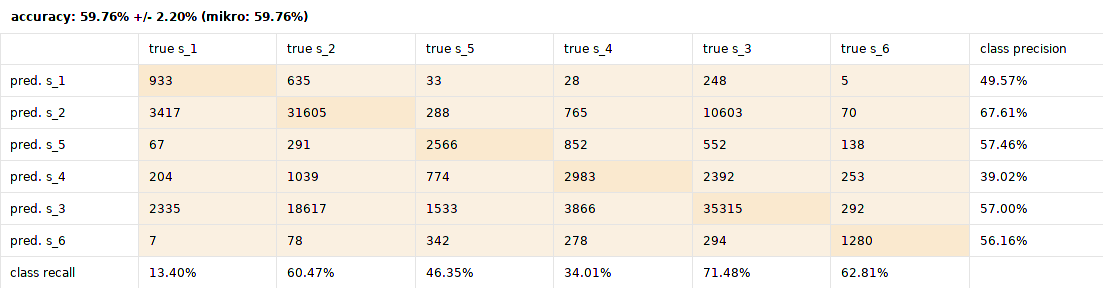
\includegraphics[scale = 0.4]{src/pic/NN_without_vector.png}
		\caption{An example of a neural net trained without person vector data.}
		\label{fig: NN without vector}
	\end{figure}
	\vspace*{-1.5em}
	
	For each neural net we are using equally distributed data sets with 100, 200 and the maximal amount of 595 individuals per strata. For every neural net and every set size, we perform 5 independent runs and calculate the average over those accuracy values in order to have a sophisticated, comparable statement. 
	\setlength\tabcolsep{.2cm}
	\begin{figure}[H]
		\centering
		\begin{tabular}{|c|c|c|c|c|c|}
			\hline
			&   \#    &        & \multicolumn{3}{c|}{Set size} \\
			Name           & Neurons &   AG   &  100  &  200  &      595      \\ \hline
			$\mathcal{N}_5$      &    5    & \xmark & 60.03 & 59.92 &     60.18     \\
			$\mathcal{N}_5^\star$   &    5    & \cmark & 87.6  & 89.7  &     71.05     \\
			$\mathcal{N}_{10}$    &   10    & \xmark & 75.83 & 73.54 &     69.56     \\
			$\mathcal{N}_{10}^\star$ &   10    & \cmark & 92.93 & 93.48 &     74.58     \\		
			%		$\mathcal{N}_{10}^\star$ &   10    & \cmark & 88.33 {\small $\pm$7.49} & 90.67{\small $\pm$2.81} & 92.14 {\small $\pm$ 2.59} \\
			$\mathcal{N}_{20}$    &   20    & \xmark & 75.45 & 71.14 &     61.87     \\
			$\mathcal{N}_{20}^\star$ &   20    & \cmark & 92.87 & 94.4  &     78.32     \\ \hline
		\end{tabular}
		\caption{The accuracy values of the neural nets}
		\label{tab: nn-accuracy}
		% mittels deep-learning-vector-average
	\end{figure}
	
	%TODO: recompute
	The size of larger nets, in terms of neurons, is counter-productive, since, if we take 50 neurons per layer, we have $14 \cdot 50^4 \cdot 6 < 849 \cdot 50^4 \cdot 6 \approxeq 31.837.500.000$ synapses for which the input dataset would be too small to perform sufficient training.\\